\chapter{Anwendungsaufbau}
\label{ch:anwendungsaufbau}
Im Folgenden wollen wir den Aufbau der implementierten Software bezüglich ihrer Funktionalität und der getroffenen Designentscheidungen der autonomen Kameraführung betrachten. 
\section{Programmaufbau}
\begin{figure}[h]
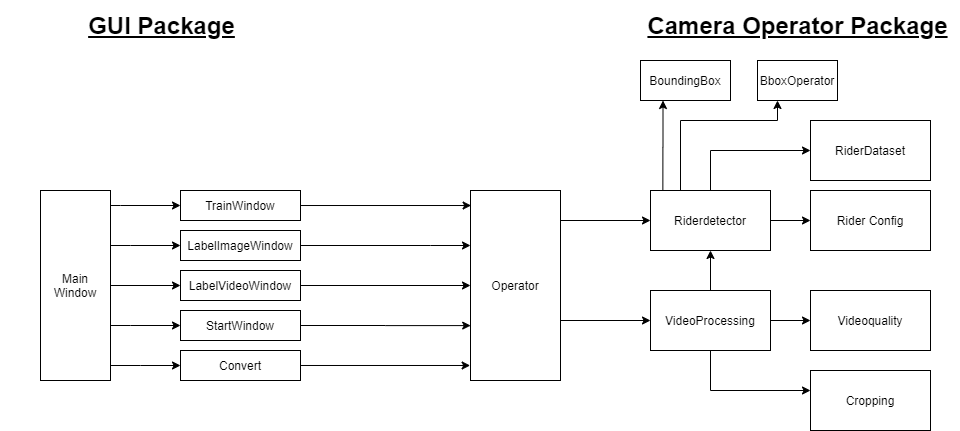
\includegraphics[width=\textwidth]{./img/Klassendiagramm.png}
\caption{Klassendiagramm vom Smart Camera Operator}
\label{fig:Klassendiagramm}
\end{figure}
Wir haben Frontend und Backend separiert, wobei die Klasse des Operators die Schnittstelle bildet. Für die Umsetzung der GUI wurde das Prinzip des Model View Controllers verwendet, um die Nutzereingaben effizient verarbeiten zu können. Der Smart Camera Operator besteht aus den beiden Hauptkomponenten des Detektors, der Training und Object Detection übernimmt, sowie des Videoverarbeitung, welche das Tracking eines Reiterpaares und die Videoqualität umfasst.

\newpage

\section{Video-Pipeline}

\begin{figure}[H]
\centering
\resizebox{.9\linewidth}{!}{
\begin{tikzpicture}[>=stealth,shorten >=1pt,auto,node distance=1cm,scale=1, transform shape,align=center,minimum size=7em,text width=6em,line width=0.14 em,rounded corners]


 \node[draw,fill=lightgray,fill opacity=0.3,text opacity=1] (A) at (0,0) 
 {Eingabevideo};
 \node[draw,right =of A,fill=lightgray,fill opacity=0.3,text opacity=1] (B) 
 {Extraktion der Frames};
 \node[draw,right =of B,fill=lightgray,fill opacity=0.3,text opacity=1] (C)
 {Detektion der Bounding Boxen von Reitern und Pferden};
 \node[draw,right =of C,fill=lightgray,fill opacity=0.3,text opacity=1] (D) 
 {Berechnung der Gesamtbox aller Reiterpaare};
 \node[draw, below =of D,fill=lightgray,fill opacity=0.3,text opacity=1] (E) 
 {Ratio der Box anpassen};
 \node[draw, below =of C,fill=lightgray,fill opacity=0.3,text opacity=1] (F) 
 {Sonderfälle am Bildrand beachten} ;
 \node[draw, below =of B,fill=lightgray,fill opacity=0.3,text opacity=1] (G) 
 {Zuschneiden der Frames} ;
 \node[draw, below =of A,fill=lightgray,fill opacity=0.3,text opacity=1] (H) 
 {Ausgabevideo} ;

 \path [->] (A) edge node[left] {} (B);
 \path [->](B) edge node[left] {} (C);
 \path [->](C) edge node[left] {} (D);
 \path [->](D) edge node[left] {} (E);
 \path [->](E) edge node[right] {} (F);
 \path [->](F) edge node[left] {} (G);
 \path [->](G) edge node[below] {} (H); 
\end{tikzpicture}
}

\caption{Video-Pipeline Phase 2}
\label{fig:VideoPipelinePhase2}
\end{figure}
\begin{figure}[H]
\centering
\resizebox{.9\linewidth}{!}{
\begin{tikzpicture}[>=stealth,shorten >=1pt,auto,node distance=1cm,scale=1, transform shape,align=center,,minimum size=7em,text width=6em,line width=0.14 em,rounded corners]

 \node[draw,fill=lightgray,fill opacity=0.3,text opacity=1] (A) at (0,0) 
 {Eingabevideo};
 \node[draw,right =of A,fill=lightgray,fill opacity=0.3,text opacity=1] (B) 
 {Extraktion der Frames};
 \node[draw,right =of B,fill=lightgray,fill opacity=0.3,text opacity=1] (C)
 {Verkleinern der Frames};
 \node[draw,right =of C,fill=lightgray,fill opacity=0.3,text opacity=1] (D)
 {Detektion der Bounding Boxen von Reitern und Pferden};
	%second row
	\node[draw,below =of D,fill=lightgray,fill opacity=0.3,text opacity=1] (E)
 {Vergrößern der detektierten Boxen}; 
 \node[draw,below =of C,fill=lightgray,fill opacity=0.3,text opacity=1] (F) 
 {Berechnung der Boxen von Reiterpaaren};
 \node[draw,below =of B,fill=lightgray,fill opacity=0.3,text opacity=1] (G)
 {Auswahl und Tracken eines Reiterpaares};
 \node[draw, below =of A,fill=lightgray,fill opacity=0.3,text opacity=1] (H) 
 {Ratio der Box anpassen};
 %third row
 \node[draw, below =of H,fill=lightgray,fill opacity=0.3,text opacity=1] (I) 
 {Sonderfälle am Bildrand beachten} ;
 \node[draw,below =of G,fill=lightgray,fill opacity=0.3,text opacity=1] (J)
 {Glätten aller Boxen};
 \node[draw, below =of F,fill=lightgray,fill opacity=0.3,text opacity=1] (K) 
 {Zuschneiden der Frames} ;
 \node[draw,below =of E,fill=lightgray,fill opacity=0.3,text opacity=1] (L)
 {Ausgabevideo};

 \path [->] (A) edge node[left] {} (B);
 \path [->](B) edge node[left] {} (C);
 \path [->](C) edge node[left] {} (D);
 \path [->](D) edge node[left] {} (E);
 \path [->](E) edge node[right] {} (F);
 \path [->](F) edge node[left] {} (G);
 \path [->](G) edge node[below] {} (H); 
 \path [->](H) edge node[below] {} (I); 
 \path [->](I) edge node[below] {} (J); 
 \path [->](J) edge node[below] {} (K); 
 \path [->](K) edge node[below] {} (L); 
\end{tikzpicture}
}

\caption{Video-Pipeline Phase 3}
\label{fig:VideoPipelinePhase3}
\end{figure}

Anhand der Ziele von den Phasen zwei und drei haben wir die Vorgehensweise mit einer Video-Pipeline geplant, welche wir dann schrittweise mit sinnvoller Aufgabenteilung umsetzen konnten. Die erste Version (Abb. \ref{fig:VideoPipelinePhase2}) umfasst dabei lediglich die grundlegenden Funktionen, die für das sinnvolle Bestimmen der ROI nötig sind. So wird hier pro Frame eines Videos für alle detektierten Reiterpaare ein gemeinsamer Bildausschnitt berechnet und diese ROI zu einem Ausgabevideo zusammengefügt.
Diese Video-Pipeline konnten wir dann in der dritten Phase (Abb. \ref{fig:VideoPipelinePhase3}) um weiter Aspekte erweitern, wobei diesmal der Fokus auf der Qualität des Ausgabevideos lag. Die Detektion konnte auf Frames mit geringerer Auflösung schneller durchgeführt werden, weshalb die Größe der gefundenen Boxen anschließen angepasst werden musste. Anstatt dem vorherigen Ansatz alle Reiterpaare zu verfolgen, wird nun ein einzelnes davon ausgewählt. Die Qualität des Ausgabevideos wird durch weniger sprunghafte Unterschiede in der Größe der aufeinanderfolgen ROI verbessert, sodass der Bildfluss flüssiger wird.

\section{Zustandsautomat}

Folgender Moore-Automat (Abb. \ref{fig:MoorAutomat}) soll zeigen, wie unser Smart Camera Operator idealerweise funktionieren soll.
Der Automat startet im \emph{missing} Zustand.
Die Transitionen \emph{gefunden} und \emph{nicht gefunden} beziehen sich auf ein Reiterpaar, das im Bild gefunden wurde - oder nicht.
In der unteren Hälfte jedes Zustands befinden sich die Aktionen, die durchgeführt werden solange sich der Automat in dem Zustand befindet.

\begin{figure}[h]
\centering
\resizebox{.9\linewidth}{!}{
\begin{tikzpicture}[->,>=stealth',shorten >=1pt,auto,node distance=6cm,thick,
	every node/.style={font=\sffamily\bfseries},
	main node/.style={rounded corners,fill=lightgray!20,draw,font=\sffamily}]

	\node[main node, rectangle split, rectangle split parts=2] (A) at (0,0)
	{\textbf{missing} \nodepart{second}zoom out, detect };
	\node[main node, rectangle split, rectangle split parts=2] (B) [right of =A]
	{\textbf{found} \nodepart{second} zoom in, track};
	\node[main node, rectangle split, rectangle split parts=2] (C) [right of =B]
	{\textbf{lost} \nodepart{second} stop track, detect};
 
	\path [->] (A) edge node[above]	 	{gefunden} 			(B);
	\path [->] (B) edge node[above]	 	{nicht gefunden}		(C);
	\path [->] (C) edge[bend right] node[above] {gefunden} 			(B)
		 edge[bend left] node[below] 	{nicht gefunden}		(A);

\end{tikzpicture}
}
\caption{Zustandsautomat vom Smart Camera Operator}
\label{fig:MoorAutomat}
\end{figure}
